% !TeX spellcheck = en_GB

\section{Monitor Pipeline}
\label{sec:concept:pipeline}

\begin{itemize}
	\item goal == monitor KNX traffic
	\item notion of \emph{project} is used to differentiate unique, not comparable KNX networks. Can be seen as a common prefix for everything which need to be named internally.
	\item monitoring should include the whole network/world view
	\item monitoring needs to be distributed, so Line Couplers can be configured properly
	\item monitoring is done by agents
	\item agents will send data gather over a time window to the collector (ref to neflow terminology)
	\item time windows of agents are synchronised (by the collector) to make data analysis more reliable
	\item agents send gathered data to collector via KNX network
	\item collector stores windows immediately in InfluxDB
	\item collector checks regularly the InfluxDB, if all agents send in their time window
	\item if so the collector relays all windows, describing the same time slot (+/- a couple seconds), to the analyser modules
	\item if not all windows are in by specified timeout (10s or so) they are relayed anyway
	\item bundled windows are distributed by pub-sub-server independently to different analytical modules
	\item analytical modules compare the windows to a base-line model (in different fashions)
\end{itemize}

\begin{figure}[h]
	\centering
	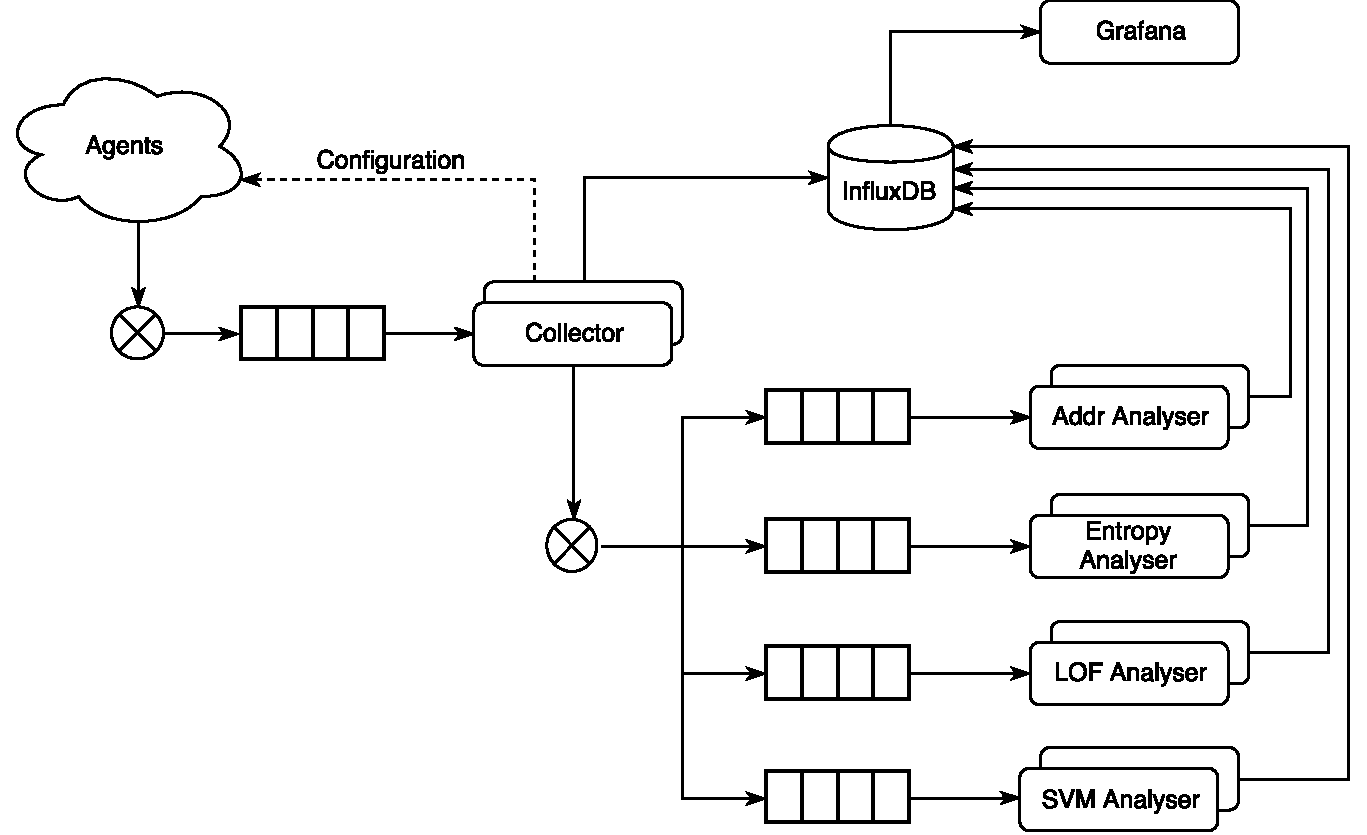
\includegraphics[width=\textwidth]{figures/300-concept-architecture.pdf}
	\caption[Pipeline Architecture]{Architecture of the monitoring pipeline}
	\label{fig:concept:architecture}
\end{figure}

\section{Design of Netflow Agent}
\label{sec:concept:agent}

\begin{itemize}
	\item dedicated device
	\item sits in each or strategic important lines
	\item listens to bypassing traffic and aggregates it
	\item \alert{Critical to describe the difference to original netflow concept/idea here and why this decision was made}
		\subitem netflow is very IP oriented, where protocols include normally connections (TCP) or at least multiple steps/packets
		\subitem this provides a basis on which aggregation/grouping can be performed
		\subitem basically no flow (multi step protocols) in \gls{knx} during normal operation (besides configuration phase in \gls{knx})
		\subitem therefore gather statistical distribution of features on \gls{knx} \gls{telegram} over a given time span (window length)
		\subitem time span/window length should be configurable by the collector, so it can be adjusted according to network utilisation
		\subitem window length still needs to be synchronised among all agents to be able to use all aggregated agent windows in a world model
		\subitem further \gls{knx} can only transport 255 Bytes max in one telegram -> serious size restrictions
	\item after timeout gathered/aggregated data is send via \gls{knx} \gls{telegram} to the collector
	\item window consists
		\subitem meta data (timestamps, window lengths)
		\subitem absolute counter of how often an specific feature appeared in a window
			\begin{itemize}
				\item specific source address
				\item specific destination address
				\item apci value
				\item a specific payload length
				\item a specific \gls{hops}
			\end{itemize}
		\subitem checksum, and possibly signature
	\item window is encoded in a binary format to fit in the 255 Bytes
\end{itemize}

\section{The Collector Module}
\label{sec:concept:collector}

\begin{itemize}
	\item responsible for
		\subitem collecting data from agents through the \gls{knx} network
		\subitem storing raw time windows in \gls{influxdb}
		\subitem relaying raw, synchronised time windows to analytical modules
	\item listens to a single message queue containing time windows from all agents assigned to the same project
	\item agents must have unique names within one project
	\item windows are parsed and then submitted into the \gls{influxdb}, tagged with the agent-name and the project
	\item window is split into different measurements (tables) determined by the \gls{knx} fields observed.
	\item one additional measurement (table) \code{agent-status}, representing general status information
		\subitem timely length of the window
		\subitem end timestamp of the window
		\subitem boolean if window was relayed or not
	\item collector regularly checks the \gls{influxdb} for unrelayed windows (latest ones first)
	\item windows are grouped by time slot
	\item if all agents have submitted a window for a specific timeslot these windows are bundled and relayed to the analyser message exchange (cf.~Figure~\ref{fig:concept:architecture})
	\item for all successfully relayed windows set the \code{realayed} flag in the \code{agent-status} measurement to \code{true}
\end{itemize}

\section{Analyser Modules}
\label{sec:concept:anal}

\begin{itemize}
	\item 2 phases
	\item distinguished learning phase
	\item during learning phase the analyser module accesses directly the \gls{influxdb} for a specified time range
	\item group windows by time equal to the functionality of the collector
	\item construct \gls{vect} to train base model
	\item save base model in the filesystem
	
	\item during normal (analytical) operation
	\item accept grouped windows from collector via message exchange
	\item compares current window groups to base model to detect anomalies
	\item results of this analysis are stored back into the \gls{influxdb} as a separate \gls{idbmeasurement}
\end{itemize}

\subsection{The Address Analyser}
\label{sec:concept:anal:addr}

\begin{itemize}
	\item purpose is to detect new (novel) device addresses
	\item cf. new device attack
	\item during the learning phase it logs all occurring source and destination addresses per agent
	\item in the analytical phase it compares all source and destination addresses in a window with addresses (base model) accumulated in the training phase
	\item output \glspl{idbmeasurement}: \code{unknown\_src\_addr}, \code{unknown\_src\_telegrams}, \code{unknown\_dest\_addr}, \code{unknown\_dest\_telegrams}, \code{unknown\_addr}, \code{unknown\_telegrams}
\end{itemize}

\subsection{The \Glsdesc{lof} Analyser}
\label{sec:concept:anal:lof}

\begin{itemize}
	\item cf.~Section~\ref{sec:background:network:novelty:lof}
	\item proximity based technique (cf.~Section~\ref{sec:background:network:novelty:prox})
	\item tries to determine if a window represents normal behaviour
	\item both for local and world view
	\item builds feature vector out of
		\subitem normalized seconds since the beginning of the year
		\subitem source addresses
		\subitem destination addresses
		\subitem priority distribution
		\subitem hop count distribution
		\subitem payload length distribution
		\subitem \gls{apci} usage distribution
	\item time sensitivity/seasonal sensitivity is archived by including the relative timepoint in the current year
	\item training different model for different seasons is not necessary since \gls{lof} is a proximity base approach
\end{itemize}

\subsection{The Entropy Analyser}
\label{sec:concept:anal:entropy}

\begin{figure}[h]
	\centering
	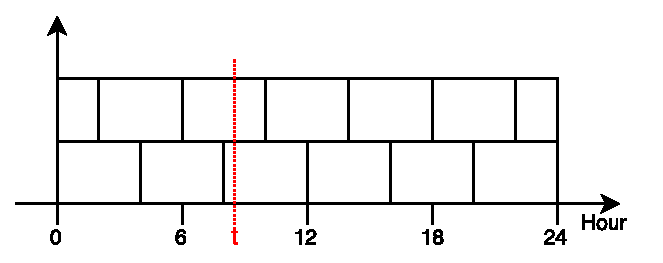
\includegraphics[]{figures/300-time-slots.pdf}
	\caption{Example of shifted time slots used in the entropy analyser module.}
	\label{fig:concept:time-slots}
\end{figure}

\begin{itemize}
	\item cf.~Section~\ref{sec:background:network:novelty:stat}
	\item statistical approach
	\item base model is trained using distribution of the \gls{pmf}
		\subitem determine statistical distribution per dimension in feature vector
	\item determine distribution for local (per agent) and world view
	\item to incorporate different seasons multiple base models are trained 
	\item the seasonal time range (day, week, year) is separated into slots
	\item amount of slots is doubled with half a slot length offset, so 2 slots apply per time point cf. Figure~\ref{fig:concept:time-slots}
	\item mitigates issues with artificial break on slot change
	\item feature vector
		\subitem source addresses
		\subitem destination addresses
		\subitem priority distribution
		\subitem hop count distribution
		\subitem payload length distribution
		\subitem \gls{apci} usage distribution
	\item entropy/information gain is calculated for the current distribution of the feature vector compared to the respectively base model
	\item individual entropies are summed up and stored in the \gls{influxdb} (additional to the individual entropies)
\end{itemize}

\section{Monitoring and Alerting}
\label{sec:concept:mon}

\begin{itemize}
	\item using \gls{grafana}
	\item visualise basic time series like amount of packets per agent
	\item visualise and monitor output from analyser modules
		\subitem should stay below certain threshold
	\item use internal alerting function
	\item benefits
		\subitem use existing, proven solution
		\subitem gain features for free (auth, alerting, graphing, etc)
		\subitem integrate with metrics from other sources
	\item decoupled from analyse modules
	\item good integration with \gls{influxdb}
\end{itemize}
